\section{已审计的系统诊断}
\label{app:system-diagnostics}

\begin{table}[!htbp]
\caption{冻结路径的执行状态。只有完成且通过严格配对验证的行才能进入最终
结果表。}
\label{tab:audited-progress}
\centering
\resizebox{\linewidth}{!}{%
\begin{tabular}{lrrrl}
\toprule
评测 & 严格配对 & 覆盖范围 & 保持率 & 状态 \\
\midrule
Llama official-middle LongBench & 3,750 / 3,750 &
16 个任务 & 99.881\% & 已完成 \\
LongBench selector 筛查 & 160 / 160 &
16 任务，每任务 10 条 & 99.789\% & 已完成 \\
早期门控消融 LongBench 筛查 & 160 / 160 &
16 任务，每任务 10 条 & 100.145\% & 已完成 \\
原生 128K Fast causal PPL & 384 / 384 &
6 个主题/seed case & 96.319\% & 已完成 \\
原生 128K Robust causal PPL & 768 / 768 &
12 个主题/seed case & 99.805\% & 已完成 \\
长度门控 General LongBench 筛查 & 80 / 80 &
16 任务，每任务 5 条 & 101.469\% & 已完成 \\
Targeted RULER 8K--64K & 91 / 91 &
13 任务，每格 2/2/2/1 条 & 99.928\% & 已完成 \\
\bottomrule
\end{tabular}}
\end{table}

已完成 Llama 实验的 Full/\method macro 为 .459398/.458852。macro
difference 的 paired-bootstrap 区间为 [$-.002647$, $.001591$]，保持率
区间为 [99.424\%, 100.347\%]。finalizer 已验证全部 3,750 个严格 pair、
16 个任务、冻结方法字段及 source hash。
Targeted RULER 的 Full/\method macro 为 .884776/.884135，paired-bootstrap
保持率区间为 [99.559\%, 100.294\%]。91 个 pair 覆盖 8/16/32/64K 的全部
13 个注册任务，但每个任务与长度只有 2/2/2/1 条，因此它是机制筛查，不能
替代正式 RULER 大表。

修正后的原生 128K 审计每个 case 使用 64 个配对 target token。Fast 的六个
同 seed case pooled 保持率为 96.319\%，最差为 91.100\%。Robust rank-16
INT4 使用冻结的 $\alpha=.5$，覆盖上述 case 与六个新 seed；99.805\% pooled
保持率的确定性 20,000 次 case-bootstrap 区间为 [99.100\%,100.499\%]，最差
为 96.980\%。实验没有触发 Full fallback。
在 80-pair 短 LongBench 筛查中，always-on Robust 保持 98.924\%，早期
长度门控 General 消融保持 101.469\%，paired-bootstrap 区间为
[99.249\%,104.449\%]。
在另一组用于公开方法对照的 160 pair 上，General 得分 .453676，Full 为
.453019，保持率 100.145\%，paired-sample 区间为 [97.915\%,102.051\%]。
80-pair 实验隔离长度门控作用；160-pair 实验审计注册部署路径与公开 selector
对照的质量。

\begin{table}[!htbp]
\caption{RTX 3090 上的 GQA-4 fused Query-preparation 验证。数值是注册
4K/32K trial 的中位数。数值检查要求 Query code 完全一致、proxy-score
NRMSE 为零、top-$k$ set 完全一致，且 sparse output cosine 高于 .999。}
\label{tab:qfused-validation}
\centering
\begin{tabular}{lrrrr}
\toprule
模型 dtype & Query prepare & 完整选择 & Top-$k$ recall &
Output cosine \\
\midrule
FP16 & 1.547$\times$ & 1.204$\times$ & 100\% & $>.999999$ \\
BF16 & 1.755$\times$ & 1.275$\times$ & 100\% & $>.999999$ \\
\bottomrule
\end{tabular}
\end{table}

该 fused kernel 并非普适更快：当每个 KV head 映射八个 Query head 时，
32K 完整选择在 FP16/BF16 下约为 .883/.806$\times$。因此本文只把它用于
目标模型的 GQA-4 路径。八样本真实 LongBench smoke test 确认所有稀疏层均
执行 fused path，预测相对 reference path 的 exact match 为 87.5\%，平均
task score 改变量为 $-0.00213$；开启 diagnostics 的 smoke timing 不作为
速度结果。

\begin{table}[!htbp]
\caption{RTX 3090 上冻结的原生 MHA FP16 attention 路径。Full 使用不复制 KV
的原生 MHA SDPA；\method 包含 Query 准备、sampled-quantile 混合位宽扫描、
候选压缩和精确稀疏 QK--softmax--AV。}
\label{tab:length-diagnostic}
\centering
\begin{tabular}{rrrrr}
\toprule
长度 & Active/head & Full ms & \method ms & 加速 \\
\midrule
8K & 504 & .1692 & .1386 & 1.22$\times$ \\
16K & 980 & .3186 & .1946 & 1.64$\times$ \\
32K & 1,332 & .6157 & .2312 & 2.66$\times$ \\
64K & 1,288 & 1.2031 & .2684 & 4.48$\times$ \\
128K & 1,282 & 2.3745 & .3810 & 6.23$\times$ \\
\bottomrule
\end{tabular}
\end{table}

计时形状为 batch one、32 个 Query head、32 个 KV head 和 $d=128$。每个点取
三个 seed、六次同卡运行的中位数，包含 20 次 warmup 和 80 次正式迭代。实际
mixed-bit 索引平均占 FP16 K+V 的 5.525\%，5.859\% 是硬上限。历史索引构建和
ValueSketch 不计入。split 8 与其 reference 完全一致；更快的 split 16 因
128K 输出余弦最低约 .80 而被废弃。

FIER 的审计 CUDA port 只支持 FP16，因此单独报告同 dtype 实验，不把它
混入上面的 BF16 表。

\begin{table}[!htbp]
\caption{RTX 3090 上确定性 full-top-$k$ selector 的 FP16 完整 attention
直接调用。Active-token 预算与 exact sparse consumer 相同。FIER 是审计过的
RTN-1 g32 忠实 port，并非原作者 runtime 的测速声明。}
\label{tab:fier-direct-fp16}
\centering
\begin{tabular}{rrrrrr}
\toprule
长度 & Full ms & \method ms & FIER ms & \method 加速 & FIER 加速 \\
\midrule
8K & .173 & .229 & .210 & .75$\times$ & .82$\times$ \\
16K & .321 & .263 & .281 & 1.22$\times$ & 1.14$\times$ \\
32K & .632 & .272 & .357 & 2.33$\times$ & 1.77$\times$ \\
64K & 1.228 & .342 & .575 & 3.59$\times$ & 2.14$\times$ \\
128K & 2.586 & .455 & 1.001 & 5.68$\times$ & 2.58$\times$ \\
\bottomrule
\end{tabular}
\end{table}

\begin{table}[!htbp]
\caption{RTX 3090 上 Llama-3.1-8B 的直接计时。Steady 是完整 model forward；
Decode 包围完整 32-token 生成区间并包含方法初始化；Request 还包含 prefill。}
\label{tab:direct-system-timing}
\centering
\begin{tabular}{rrrrr}
\toprule
长度 & Steady & 32-token decode & Request & 质量保持率 \\
\midrule
8K & .843$\times$ & .196$\times$ & .484$\times$ & 96.94\% \\
16K & 1.217$\times$ & .292$\times$ & .680$\times$ & 100.70\% \\
32K & 1.552$\times$ & .452$\times$ & .880$\times$ & 96.65\% \\
64K & 2.656$\times$ & .767$\times$ & .980$\times$ & 98.84\% \\
128K & 4.937$\times$ & 1.384$\times$ & 1.011$\times$ & 97.86\% \\
\bottomrule
\end{tabular}
\end{table}

不同长度使用不同 PPL 窗口，因此这里只诊断执行，不构成受控质量长度曲线。
但系统 crossover 很清晰：attention 与整模型 steady 约在 16K 出现收益，
32-token decode 直到约 128K 才加速，而请求级在 128K 也仅略高于 1。

\begin{figure}[!htbp]
  \centering
  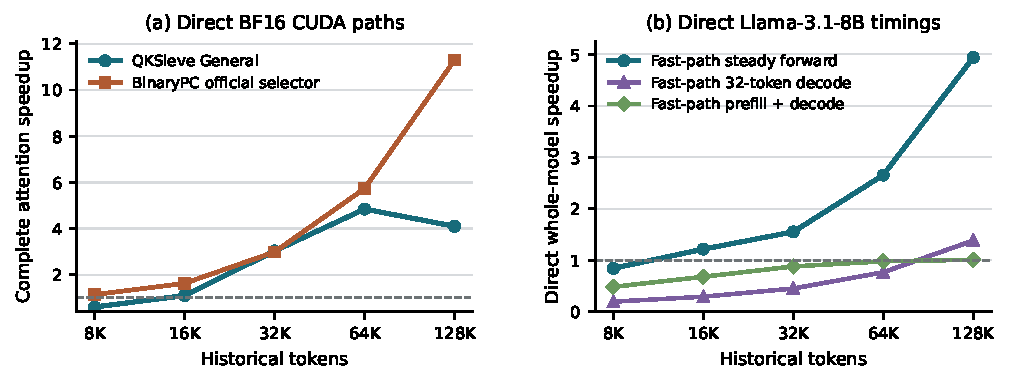
\includegraphics[width=\linewidth]{figures/qksieve_system_diagnostics.pdf}
  \caption{RTX 3090 直接测量。左：\method 与 BinaryPC 发布 selector 的完整
  BF16 单层 attention call。右：Fast 路径的 Llama-3.1-8B steady forward、
  直接测量的 32-token decode 区间和 prefill-plus-decode 请求；右图只是
  crossover 诊断，不是 General 配置的速度声明。没有曲线由独立阶段求和构造。}
  \label{fig:speed}
\end{figure}

\begin{table}[!htbp]
\caption{RTX 3090 上冻结的原生 MHA FP16 组件计时。各组件独立调用以定位
瓶颈，不能通过求和重建直接计时的完整路径。}
\label{tab:deployment-breakdown}
\centering
\begin{tabular}{rrrrr}
\toprule
长度 & Query 准备 & Selector scan & Sparse attention & 完整路径 \\
\midrule
8K & .0336 & .0365 & .0438 & .1386 \\
16K & .0335 & .0468 & .0910 & .1946 \\
32K & .0299 & .0634 & .1107 & .2312 \\
64K & .0302 & .0999 & .1186 & .2684 \\
128K & .0303 & .1673 & .1630 & .3810 \\
\bottomrule
\end{tabular}
\end{table}

Query 准备几乎不随长度变化。128K 下 packed scan 和精确稀疏 consumer 占主导；
候选物化、gather 和 kernel launch 解释独立阶段与完整调用之间的差值。512 个
quantile sample 上限专门降低长上下文 selector 开销，但不改变 packed-index
线性扫描本身。

\begin{table}[!htbp]
\caption{RTX 3090 上较早的 GQA-4 QKSieve Fast--Robust BF16 直接测速。完整路径直接计时；
scan 和 consumer 行为独立调用诊断，不参与求和。Robust 使用 rank-16
block-affine INT4 Value 系数与 $\alpha=.5$。}
\label{tab:robust-direct-timing}
\centering
\begin{tabular}{lrr}
\toprule
128K 直接操作 & 时间 (ms) & 相对 Full \\
\midrule
Full attention & 2.451 & 1.000$\times$ \\
Fast 完整 attention & .398 & 6.161$\times$ \\
Robust 完整 attention & .595 & 4.119$\times$ \\
General 条件分支完整调用 & .598 & 4.100$\times$ \\
Robust Key+Value-tail scan & .347 & -- \\
Robust exact-selected-plus-tail consumer & .190 & -- \\
\bottomrule
\end{tabular}
\end{table}

Robust 的逐 token index 包括 240 个 Key bit、64 个 Value coefficient bit 和
2 个摊销 block-metadata bit，总计为 FP16 K+V 的 7.471\%。其 12-case 整模型
稳态加速几何平均为 3.224$\times$；把一次性初始化摊销到直接测量的 64 个 decode
token 后为 1.125$\times$。它比 Fast 慢，但与独立验证的原生 128K 稳健质量配对。

\begin{table}[!htbp]
\caption{固定每 head 1,280 个 exact-attention token 时的长历史物理 CUDA
attention scaling。256K/512K 行汇总 36 个 Qwen3-style layer，不含非
attention 模型工作与首次 index construction。严格 256K 诊断表明固定
1,280 的冻结 proxy 配置质量不合格；512K 也超出模型原生长度，因此这些行
只隔离低预算算子 scaling。}
\label{tab:long-history-attention}
\centering
\begin{tabular}{lrrr}
\toprule
History & Full SDPA & \method & 加速 \\
\midrule
128K，单层 & 2.439 ms & .360 ms & 6.78$\times$ \\
256K，$B=1280$ & 175.008 ms & 12.650 ms & 13.83$\times$ \\
512K，$B=1280$ & 380.282 ms & 17.513 ms & 21.71$\times$ \\
\bottomrule
\end{tabular}
\end{table}

\begin{table}[!htbp]
\caption{单张 RTX 3090 上的高保真长历史 attention timing。\method 使用
24\% active token，并包含 Query projection/quantization、low-bit
retrieval、sampled quantile selection 与 exact sparse attention。
pre-expanded baseline 不计 GQA replication；HF-style baseline 计入
\texttt{repeat\_kv} 与 SDPA。时间汇总 36 层，不含 index construction 和
非 attention 工作。}
\label{tab:long-history-highfidelity-attention}
\centering
\small
\resizebox{\linewidth}{!}{%
\begin{tabular}{lrrrrr}
\toprule
History & Pre-expanded SDPA & HF GQA+SDPA & \method &
vs pre-expanded & vs HF \\
\midrule
256K & 175.104 ms & 567.610 ms & 199.992 ms & .876$\times$ &
2.838$\times$ \\
512K & 348.520 ms & 1135.721 ms & 373.800 ms & .932$\times$ &
3.038$\times$ \\
\bottomrule
\end{tabular}}
\end{table}

高保真 sparse path 并不快于已经物化 GQA K/V 的理想 SDPA consumer；
它的实际优势来自相对真实 HF 路径省去每个 decode step 的 GQA replication。
因此本文同时报告两个分母。512K 24\% selector 使用 768 个分层样本
（$c=128$），以使 confidence capacity 不超过 16-way ragged-kernel 限制。

\begin{table}[!htbp]
\caption{四个独立打乱 20-Newsgroups 窗口上的严格原生边界 256K
causal-PPL frontier（262,080 history + 64 target/window，共 256 个严格
配对 target token）。保持率由 pooled NLL difference 计算；区间以四个
window 为 cluster bootstrap，因此仍是诊断性而非最终跨语料置信结论。}
\label{tab:256k-frontier}
\centering
\small
\resizebox{\linewidth}{!}{%
\begin{tabular}{rrrrr@{\qquad}r}
\toprule
Active & 保持率（95\% CI） & Top-1 & KL & Steady & Online \\
\midrule
7.977\% & 94.440\% [93.38, 95.68] & 78.516\% & .04365 &
5.511$\times$ & 4.925$\times$ \\
9.977\% & 96.260\% [94.53, 97.73] & 82.031\% & .03266 &
5.345$\times$ & 5.097$\times$ \\
11.927\% & 96.949\% [94.79, 98.43] & 83.984\% & .02696 &
4.453$\times$ & 4.283$\times$ \\
15.951\% & 97.418\% [95.43, 99.07] & 83.594\% & .02250 &
3.642$\times$ & 3.377$\times$ \\
20.055\% & 99.072\% [97.62, 100.55] & 84.766\% & .01349 &
2.959$\times$ & 2.887$\times$ \\
\textbf{23.958\%} & \textbf{100.250\% [99.40, 101.06]} &
\textbf{92.188\%} & \textbf{.00733} & \textbf{2.989$\times$} &
\textbf{2.911$\times$} \\
\bottomrule
\end{tabular}}
\end{table}

23.958\% 点在这些窗口上与 Full 统计匹配；略高于 100\% 不代表 sparse
attention 普遍提高模型。四次运行平均 Full/\method steady decode 为
588.942/197.019 ms/token。共同 prefill 为 1058.826 s，因此请求级速度达到
$2\times$ 约需生成 5,436 token。完整 FP16 K/V 保持 GPU resident：
``Active''表示 exact-attention compute，不表示 cache-memory retention。

\begin{table}[!htbp]
\caption{同一批严格 256K 窗口、256 个 target token 上的 oracle budget
诊断。Exact-QK 先计算所有历史 FP16 QK score，再选预算；low-bit proxy
使用冻结 QK-balanced/Key-MSE 240-bit index 和完整 proxy top-$k$。两者都
在原始 FP16 K/V 上计算最终精确 attention。}
\label{tab:256k-oracle-gap}
\centering
\small
\resizebox{\linewidth}{!}{%
\begin{tabular}{lrrrrrr}
\toprule
Selector & Exact/head & Active & Oracle mass & 保持率（95\% CI） &
Top-1 & KL \\
\midrule
Exact FP16 QK & 1,280 & .488\% & 90.002\% &
\textbf{100.240\% [99.48, 100.88]} & 90.625\% & \textbf{.00516} \\
Exact FP16 QK & 2,560 & .977\% & 93.057\% &
\textbf{100.148\% [99.54, 100.68]} & 92.969\% & \textbf{.00297} \\
Low-bit proxy & 1,280 & .488\% & -- &
80.771\% [77.84, 83.92] & 67.188\% & .24246 \\
Low-bit proxy & 2,560 & .977\% & -- &
86.132\% [84.68, 87.77] & 71.094\% & .15092 \\
\bottomrule
\end{tabular}}
\end{table}

\begin{table}[!htbp]
\caption{严格配对的 128K--256K selector crossover。两个长度使用相同冻结
QK-balanced/Key-MSE template、完整 proxy top-$k$、四个文本窗口/seed 和
256 个 target。表中为 PPL 保持率与四窗口 cluster-bootstrap 95\% 区间。}
\label{tab:128k-256k-selector-crossover}
\centering
\small
\resizebox{\linewidth}{!}{%
\begin{tabular}{lrrrr}
\toprule
History & Exact-1,280 & Proxy-1,280 & Exact-2,560 & Proxy-2,560 \\
\midrule
128K & 100.805\% [99.40, 102.23] & 98.993\% [96.53, 102.99] &
100.345\% [99.14, 101.57] & 100.005\% [97.66, 103.02] \\
256K & 100.240\% [99.48, 100.88] & 80.771\% [77.84, 83.92] &
100.148\% [99.54, 100.68] & 86.132\% [84.68, 87.77] \\
\bottomrule
\end{tabular}}
\end{table}

\begin{table}[!htbp]
\caption{top-1,280 下严格 256K 的坐标--allocation 正交拆分。所有行使用
相同四个 window、256 个 target、完整 top-$k$ 和原始 FP16 K/V exact
attention。Online decode 将一次性 selector preparation 摊入约 63 个
timed step，且不含共同 prefill。}
\label{tab:256k-selector-cause}
\centering
\small
\resizebox{\linewidth}{!}{%
\begin{tabular}{lrrrrr}
\toprule
Selector/index policy & 保持率（95\% CI） & Top-1 & KL & Steady & Online \\
\midrule
Exact FP16 QK & 100.240\% [99.48, 100.88] & 90.625\% & .00516 & -- & -- \\
冻结坐标 / 冻结 bits & 80.771\% [77.84, 83.92] & 67.188\% & .24246 &
7.785$\times$ & 6.668$\times$ \\
冻结坐标 / local bits & 89.911\% [84.13, 94.28] & 77.344\% & .13332 &
7.766$\times$ & 5.259$\times$ \\
Local 坐标 / 固定 bits & \textbf{100.443\% [99.80, 101.02]} & 91.016\% &
.00620 & 7.671$\times$ & \textbf{4.955$\times$} \\
Local 坐标 / local bits & 100.430\% [99.78, 100.99] & 91.016\% &
.00622 & \textbf{7.733$\times$} & 4.055$\times$ \\
冻结全 INT8 & 100.267\% [99.48, 100.91] & 91.016\% &
\textbf{.00508} & 1.882$\times$ & 1.846$\times$ \\
\bottomrule
\end{tabular}}
\end{table}

\begin{figure}[!htbp]
\centering
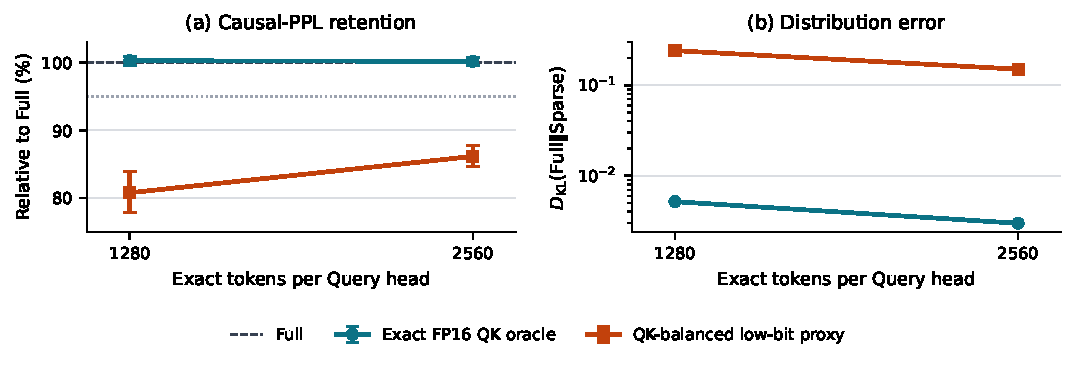
\includegraphics[width=.78\linewidth]{figures/qksieve_256k_oracle_gap.pdf}
\caption{在模型原生 256K 边界，每 Query head 只需 1,280 个 token，只要它们
由 Exact FP16 QK 选出。扩大 low-bit proxy budget 虽提高质量，仍存在显著
selection gap。误差条为四窗口 cluster-bootstrap 95\% 区间。}
\label{fig:256k-oracle-gap}
\end{figure}

这一控制实验推翻了最初的“固定 token budget 不足”解释：Exact-QK
top-1,280 在仅 .488\% active 下保持 100.24\%，但冻结 low-bit proxy 只有
80.77\%。\cref{tab:256k-selector-cause}进一步定位原因：在冻结坐标内重新
分配相同 240 bit 只恢复到 89.91\%；request-local 坐标配固定
4-1-1-1-1-1-0-0 allocation 恢复到 100.44\%，与 local 坐标加 local bits
的 100.43\% 统计匹配。因此该压力测试中的主因是坐标外推，不是预算不足；
动态 bit 在此切分上既非必要，也没有可测收益。local fixed-bit 路径仍保留
7.67$\times$ steady 与 4.96$\times$ 64-token online whole-model speed。

\begin{table}[!htbp]
\caption{一个 20-Newsgroups causal-PPL window 上的 Qwen3-4B 512K 外推
压力测试（524,256 history + 32 target）。Full PPL 已达 5510.6，因此保持率
只表示接近同一个外推 Full distribution，不是原生任务质量。}
\label{tab:512k-extrap-frontier}
\centering
\small
\begin{tabular}{rrrrrrr}
\toprule
Active & 保持率 & Top-1 & KL & Steady & Online & Count range \\
\midrule
2.951\% & 105.34\% & 93.75\% & .0978 & 10.70$\times$ &
9.00$\times$ & 5,117--33,365 \\
3.947\% & 101.63\% & 96.88\% & .0794 & 10.72$\times$ &
8.13$\times$ & 6,999--48,828 \\
4.880\% & 99.97\% & 93.75\% & .0754 & 8.98$\times$ &
7.82$\times$ & 8,805--49,759 \\
5.872\% & 98.57\% & 96.88\% & .0592 & 7.72$\times$ &
6.85$\times$ & 11,359--66,293 \\
\bottomrule
\end{tabular}
\end{table}

\begin{table}[!htbp]
\caption{160 个严格 Llama-3.1-8B 配对样本（每任务 10 条）上的 LongBench
selector 筛查。所有稀疏行使用相同 active-token schedule 和原始 KV
consumer。FIER、Quest、RaBitQ 与 SparQ 是经过审计的公式/参考实现质量对照，
不是官方优化系统测速。}
\label{tab:public-selector-quality}
\centering
\small
\begin{tabular}{lrrr}
\toprule
方法 & Index bit/token/KV-head & Active & 相对 Full 质量 \\
\midrule
Full & 0 & 100.00\% & 100.000\% \\
\method reference & 240 & 7.440\% & 99.789\% \\
FIER RTN-1 g32 reference & 256 & 7.440\% & 100.010\% \\
Quest-P16，整页加载 & 256 & 7.562\% & 92.217\% \\
RaBitQ RTN-1 reference & 224 & 7.440\% & 100.012\% \\
SparQ-R32 selector only & 0 & 7.440\% & 99.623\% \\
SparQ-R32 完整公式 & 0 & 7.440\% & 99.950\% \\
UNIQUE-P8 公式参考 & 258 & 7.494\% & 93.193\% \\
\bottomrule
\end{tabular}
\end{table}

\begin{table}[!htbp]
\caption{与发布 BinaryPC 的对比。质量使用 160 个严格 LongBench 配对样本
（每任务 10 条），仍不足以宣称显著优越；速度是在 128K、相同 $B(N)$ 与
相同 exact sparse consumer 下直接调用 BF16 单层 CUDA 路径的结果。
\method 的速度对应部署 selector，质量对应确定性 reference selector。}
\label{tab:binarypc-public-comparison}
\centering
\begin{tabular}{lrrrr}
\toprule
方法 & Index bit & Active & 相对 Full 质量 & 128K attention \\
\midrule
Full & 0 & 100.00\% & 100.000\% & 1.000$\times$ \\
BinaryPC released & 64 & 7.440\% & 99.250\% & 11.295$\times$ \\
\method & 240 & 7.440\% & 99.789\% & 6.798$\times$ \\
\bottomrule
\end{tabular}
\end{table}

FIER 行是严格同样本、同预算的 reference-quality 运行，其 quality harness
时间不用于系统速度结论。Quest-P16 按完整 16-token page 加载。SparQ 完整公式加入 $r=32$
temperature、local window、selected-mass estimate 与 mean-Value correction。
RaBitQCache 官方效率 artifact 需要 CUDA~12.8 和修改版 vLLM；当前 RTX~3090
环境使用更旧的 PyTorch CUDA runtime，因此不虚构原生 RaBitQ 速度。
当前公开的 Microsoft 仓库提供 RetroInfer，而不是原始 RetrievalAttention
的可运行 artifact。
